%!TEX program = lualatex
% Hero plate for the FlexGEMM PTC 2026 deck: one output tile of C = A @ B, with the
% epilogue applied to the accumulator before the store. Engraved treatment follows
% ~/dotfiles/.ai/skills/creating-tikz-diagrams/vintage-style.md (idea adapted from
% Foadsf/vintage-latex, CC BY-SA 4.0); geometry and content are new.
% Build: latexmk -lualatex -interaction=nonstopmode -halt-on-error tile_plate.tex
\documentclass[tikz,border=8pt]{standalone}
\usepackage{fontspec}
\usepackage{unicode-math}
\usetikzlibrary{arrows.meta,patterns,calc,decorations.pathreplacing}
\setmainfont{EBGaramond}[
  Extension=.otf, UprightFont=*-Regular, ItalicFont=*-Italic,
  BoldFont=*-Bold, Numbers={OldStyle,Proportional}]
\setmathfont{Garamond-Math.otf}
\definecolor{paper}{HTML}{F4F0E8}
\definecolor{ink}{HTML}{2B241D}
\definecolor{amber}{HTML}{97551C}
\definecolor{green}{HTML}{5F7F67}
% Transparent page: rasterize with pdftocairo -transp so the deck paper shows through.

\begin{document}
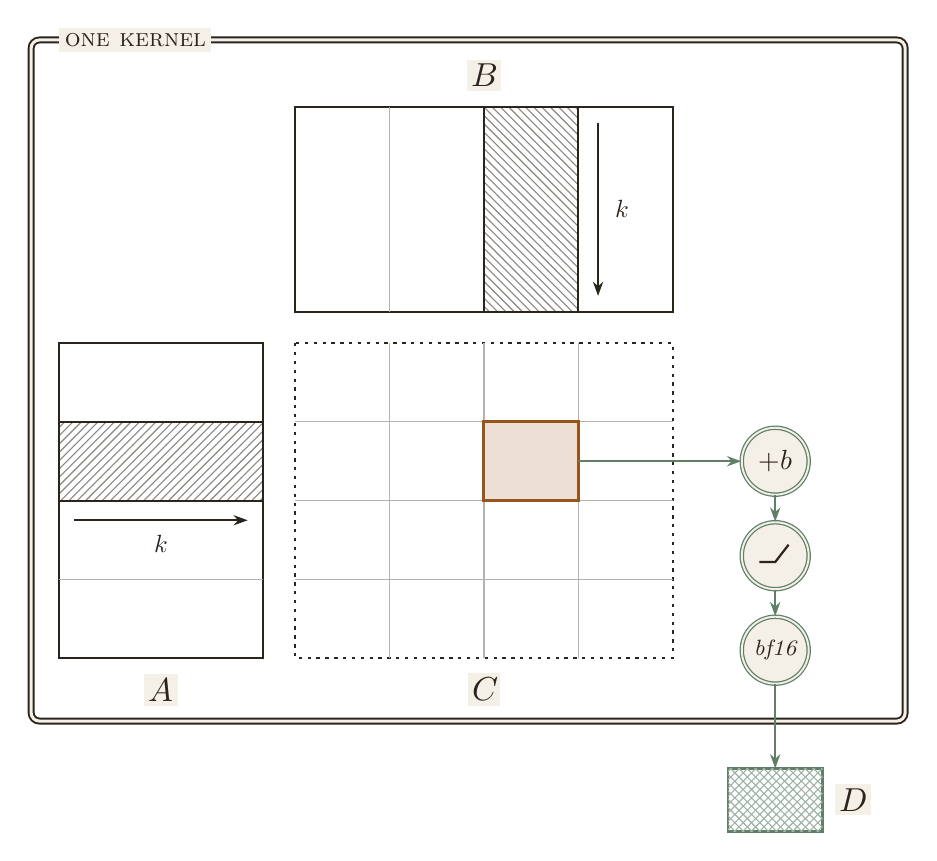
\begin{tikzpicture}[
  x=1cm, y=1cm, line width=.45pt, draw=ink, text=ink,
  flow/.style={draw=ink, line width=.6pt, -{Stealth[length=1.8mm,width=1.3mm]}},
  sym/.style={font=\itshape\large, fill=paper, inner sep=1.5pt},
]
  % Geometry: A is M x K (left), B is K x N (top), C is M x N.
  \def\M{4.0} \def\N{4.8} \def\K{2.6}
  \def\tm{1.0} \def\tn{1.2}          % output tile
  \def\ti{1} \def\tj{2}              % tile row / column index

  % Operand outlines with faint grids.
  \draw[line width=.7pt] (-\K-0.4,0) rectangle (-0.4,-\M);                 % A
  \draw[line width=.7pt] (0,\K+0.4) rectangle (\N,0.4);                    % B
  \draw[line width=.7pt, dash pattern=on 1.2pt off 2pt] (0,0) rectangle (\N,-\M);  % C: never stored
  \foreach \i in {1,...,3} \draw[ink!35] (0,-\i*\tm) -- (\N,-\i*\tm);
  \foreach \j in {1,...,3} \draw[ink!35] (\j*\tn,0) -- (\j*\tn,-\M);
  \foreach \i in {1,...,3} \draw[ink!35] (-\K-0.4,-\i*\tm) -- (-0.4,-\i*\tm);
  \foreach \j in {1,...,3} \draw[ink!35] (\j*\tn,\K+0.4) -- (\j*\tn,0.4);

  % Engraved strips: the tile's row panel of A and column panel of B.
  \fill[pattern=north east lines, pattern color=ink!55]
    (-\K-0.4,-\ti*\tm) rectangle (-0.4,-\ti*\tm-\tm);
  \fill[pattern=north west lines, pattern color=ink!55]
    (\tj*\tn,\K+0.4) rectangle (\tj*\tn+\tn,0.4);
  \draw[line width=.7pt] (-\K-0.4,-\ti*\tm) rectangle (-0.4,-\ti*\tm-\tm);
  \draw[line width=.7pt] (\tj*\tn,\K+0.4) rectangle (\tj*\tn+\tn,0.4);

  % K sweep marks along both panels.
  \draw[flow] (-\K-0.2,-\ti*\tm-\tm-0.25) -- (-0.6,-\ti*\tm-\tm-0.25);
  \draw[flow] (\tj*\tn+\tn+0.25,\K+0.2) -- (\tj*\tn+\tn+0.25,0.6);
  \node[font=\itshape\small] at (-\K/2-0.4,-\ti*\tm-\tm-0.55) {$k$};
  \node[font=\itshape\small] at (\tj*\tn+\tn+0.55,\K/2+0.4) {$k$};

  % The accumulator tile, in amber: the one thing to watch.
  \fill[amber!18] (\tj*\tn,-\ti*\tm) rectangle (\tj*\tn+\tn,-\ti*\tm-\tm);
  \draw[amber, line width=1.1pt] (\tj*\tn,-\ti*\tm) rectangle (\tj*\tn+\tn,-\ti*\tm-\tm);
  \coordinate (acc) at (\tj*\tn+\tn/2,-\ti*\tm-\tm/2);

  % The epilogue E, in green: the user's own PyTorch ops, applied to the tile in
  % registers, as a chain of engraved beads (+ captured bias, relu, cast).
  \def\ex{\N+1.3}
  \tikzset{bead/.style={circle, draw=green, double=paper, double distance=.7pt,
    line width=.45pt, fill=paper, minimum size=8.5mm, inner sep=0pt, font=\normalsize}}
  \node[bead] (b1) at (\ex,-\ti*\tm-\tm/2) {$+b$};
  \node[bead] (b2) at (\ex,-\ti*\tm-\tm/2-1.2) {};
  \draw[ink, line width=.8pt] ($(b2)+(-0.2,-0.08)$) -- ($(b2)+(0,-0.08)$) -- ($(b2)+(0.17,0.14)$);
  \node[bead, font=\footnotesize\itshape] (b3) at (\ex,-\ti*\tm-\tm/2-2.4) {bf16};
  \draw[flow, draw=green] ($(acc)+(\tn/2,0)$) -- (b1.west);
  \draw[flow, draw=green] (b1) -- (b2);
  \draw[flow, draw=green] (b2) -- (b3);
  % The slide draws the dashed flex slot and its label over this chain.

  % The kernel boundary: everything above happens inside one kernel; only D leaves.
  \draw[ink, line width=.7pt, double=paper, double distance=1.1pt, rounded corners=3pt]
    (-\K-0.75,\K+1.25) rectangle (\N+2.95,-\M-0.8);
  \node[font=\small\scshape, fill=paper, inner sep=2pt, anchor=west]
    at (-\K-0.4,\K+1.25) {one kernel};

  % D, outside the boundary: the only tensor written to memory.
  \draw[green, line width=.9pt] (\ex-0.6,-\M-1.4) rectangle (\ex+0.6,-\M-2.2);
  \fill[pattern=crosshatch, pattern color=green!60] (\ex-0.6,-\M-1.4) rectangle (\ex+0.6,-\M-2.2);
  \draw[flow, draw=green] (b3.south) -- (\ex,-\M-1.4);

  % Minimal symbols only.
  \node[sym] at (-\K/2-0.4,-\M-0.4) {$A$};
  \node[sym] at (\N/2,\K+0.8) {$B$};
  \node[sym] at (\N/2,-\M-0.4) {$C$};
  \node[sym, anchor=west] at (\ex+0.75,-\M-1.8) {$D$};
\end{tikzpicture}
\end{document}
